\documentclass[conference]{IEEEtran}
\IEEEoverridecommandlockouts
% The preceding line is only needed to identify funding in the first footnote. If that is unneeded, please comment it out.
\usepackage{cite}
\usepackage{amsmath,amssymb,amsfonts}
\usepackage{algorithmic}
\usepackage{graphicx}
\usepackage{textcomp}
\usepackage{xcolor}
\usepackage{booktabs}
\usepackage{adjustbox}
\usepackage{float}

\bibliographystyle{IEEEtran}

\def\BibTeX{{\rm B\kern-.05em{\sc i\kern-.025em b}\kern-.08em
    T\kern-.1667em\lower.7ex\hbox{E}\kern-.125emX}}
\begin{document}

\title{The Best Seat at UD}

\author{
\IEEEauthorblockN{Maxmillian Stratton, Jackson Rau, Quinlan Kraft, Braden Rogers, Kyle Wodehouse}
\IEEEauthorblockA{
University of Delaware\\
}
}

\maketitle




\section{Introduction}

Chairs and the culture of sitting down developed in Ancient Egypt \cite{egypt}. Egyptian chairs, at least those preserved in tombs, look quite different from the 21st century chair. They sat closer to the ground and were made from lavish materials on a wooden frame---far from any UD chair. Everyone has experienced the dreadful ergonomics of Smith 209. The backrest angle feels awkward for taking notes and the arm rests are egregiously high to the point where one cannot even relax the shoulders comfortably. On the other hand, Willard 319 features adjustable chairs and plentiful desk space disconnected from the chair itself. 

Experiencing both immaculate and disastrous seating raises the question: what is the best seat at UD? To answer this question (and the funnier question of what is the worst seat at UD) we need to probe the population of desks around campus. Then, once a representative sample of desk and chair parameters is collected it can be analyzed as a whole and also compared to each other to figure out how UD`s desks fare overall and if any desks are fantastic or deeply flawed.
%{M.G. Mohamed Thariq et. al, page 1} Ansari et. al 

Ergonomics researchers acknowledge the importance of ergonomics for students` experience and generally concludes sitting in fixed tables and chairs lead to strained posture and poor experiences\cite{mohamed}.  A pair of studies \cite{mohamed} \cite{Ansari} measured college students in Iran and Sri Lanka and developed chair dimensions based on their knowledge of sitting ergonomics and certain quantiles of their anthropic college student measurements. Table \ref*{tab:determinants1} shares how \cite{mohamed} determined their chair parameters and Table \ref*{tab:determinants2} shares the same information for \cite{Ansari}. Table \ref*{tab:dimension_comparison} includes the measurements \cite{mohamed} and \cite{Ansari} determined were optimal for college student desks.\footnote{the dimensions provided by \cite{mohamed} were first converted from  milimeters to centimeters before being included in Table \ref*{tab:dimension_comparison}.}




\begin{table}[htbp]
    \caption{Chair Features and Determinants from\cite{mohamed}}
    \begin{center}
    \begin{tabular}{c c}
    \toprule
    \textbf{Chair Feature} & \textbf{Determinant} \\
    \midrule
    Seat surface height & Seat height boundary case + 25 mm allowance \\
    \midrule
    Desktop height & Elbow height, sitting boundary case \\
    \midrule
    Desktop length & 50\%ile Forearm--finger tip length \\
    \midrule
    Desktop width & As per existing desktop width \\
    \bottomrule
    \end{tabular}
    \label{tab:determinants1}
    \end{center}
\end{table}

\begin{table}[htbp]
    \caption{Chair Features and Determinants from~\cite{Ansari}}
    \begin{center}
    \begin{tabular}{c c}
    \toprule
    \textbf{Chair Feature} & \textbf{Determinant} \\
    \midrule
    Seat height & 5th percentile (female) of popliteal height \\
    \midrule
    Desk height & 5th--95th percentile (all) of elbow height \\
    \midrule
    Desk length & 95th percentile (male) of elbow-fingertip length \\
    \midrule
    Desk width & 95th percentile (male) of elbow to elbow width \\
    \bottomrule
    \end{tabular}
    \label{tab:determinants2}
    \end{center}
\end{table}
    
\begin{table}[htbp]
    \caption{Comparison of Design Dimensions from ~\cite{mohamed} \& ~\cite{Ansari}}
    \begin{center}
    \begin{tabular}{c c c}
    \toprule
    \textbf{Chair Feature} & \textbf{Dimension ~\cite{mohamed} (cm)} & \textbf{Dimension ~\cite{Ansari} (cm)} \\
    \midrule
    Seat height & 44.5 & 44 \\
    \midrule
    Desk height & 22.9 & 19--29 \\
    \midrule
    Desk length & 45.3 & 51 \\
    \midrule
    Desk width & 19.8 & 65 \\
    \bottomrule
    \end{tabular}
    \label{tab:dimension_comparison}
    \end{center}
\end{table}

\pagebreak

Using the dimensions provided by the literature, desks and chairs found in common UD lecture rooms, specifically rooms classified by the central classroom inventory, may be compared to a standard and the faults of poor seats may be understood from an objective angle rather than personal experiences of uncomfort while sitting in them.




\section{Methods}

In an effort to collect the most accurate data, it’s important to adhere to the same procedure during each instance of data collection. To start, identify the building, room number, and room type that the measurements are being taken in. Next, identify the desk “type” that is being measured. When performing this step, each time you encounter a new desk “type”, add it to a reference document with an image and description to catalog all different styles of desk encountered. Doing so allows for easier data collection as descriptions and images don’t have to be repeated between rooms when the desks are of the same “type”, and can instead be generalized per desk “type”. 

Next, begin taking physical measurements of the desk. Despite the generalization for descriptions and images, it’s important to take separate data measurements per room. Even when the desks appear visually similar or the same, they could have slightly different measurements. Start by measuring the height from the floor to the tallest point of the seat of the desk (i.e. where someone would sit). Next, measure the height from the floor to the tallest point of the physical desk (i.e. the writing surface). For both of these measurements, the seat and desk surface may not be flat and/or could be at an angle, so it’s important to measure to the highest point of the surface to be consistent. Lastly, measure the width and length of the “useable” desk area (i.e. not including the armrest portion) by approximating it as a rectangle. For shared tables or desks, this can be calculated by finding the overall area and then dividing by the number of seats at the table, thus giving the usable area per person at the table. It is recommended to collect this data in a spreadsheet application with the following columns: building, room number, room type, desk type, seat height, desk height, desk width, and desk length.




\section*{Acknowledgment}

A thank you is due to any CHEG304080 student who offered feedback during our in class presentations. A specific thank you is owed to Prof. Enszer for suggesting to look at UD`s central classroom inventory.

\bibliography{zotero}   



\section*{Appendix}

\subsection{Notes on Data Storage and Analysis}

Data was stored in a shared google sheet file for accessability reasons. Analysis and visualization was completed in Jupyter Notebooks using python. As far as packages go, pandas was used to wrangle the data and matplotlib was used to create the visualizations. 

\subsection{Additional visualizations}

\begin{figure}[H]
    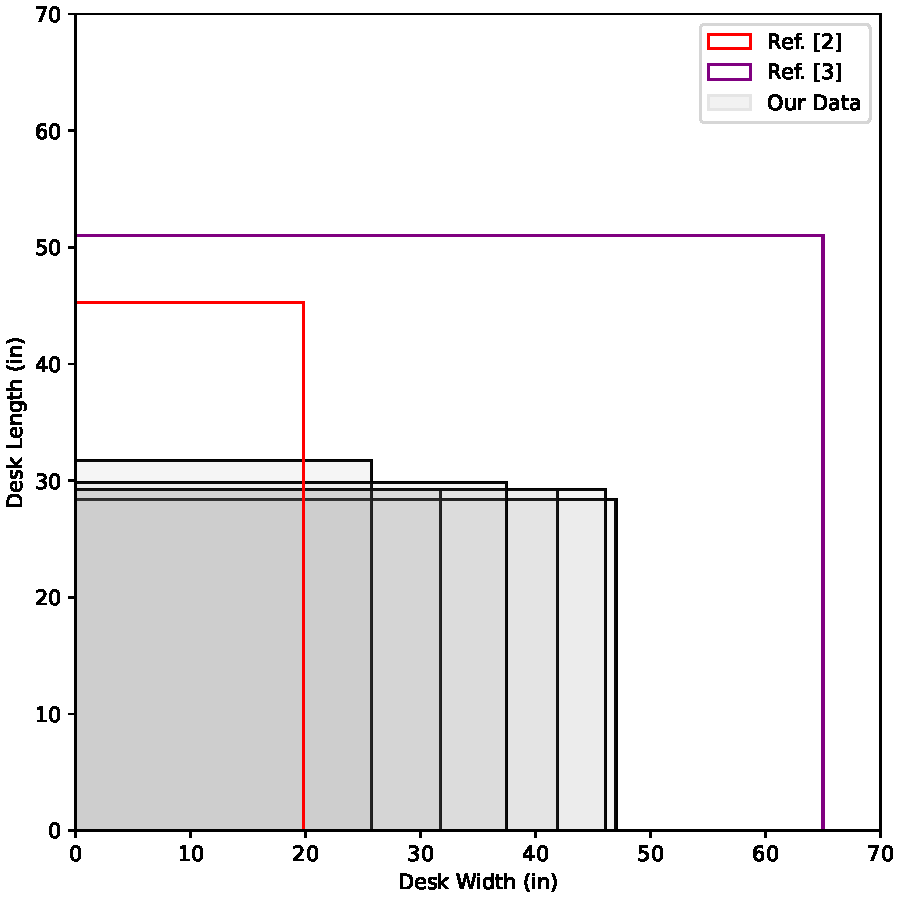
\includegraphics[width=\linewidth]{vis/rectangles.pdf}
\end{figure}

\begin{figure}[H]
    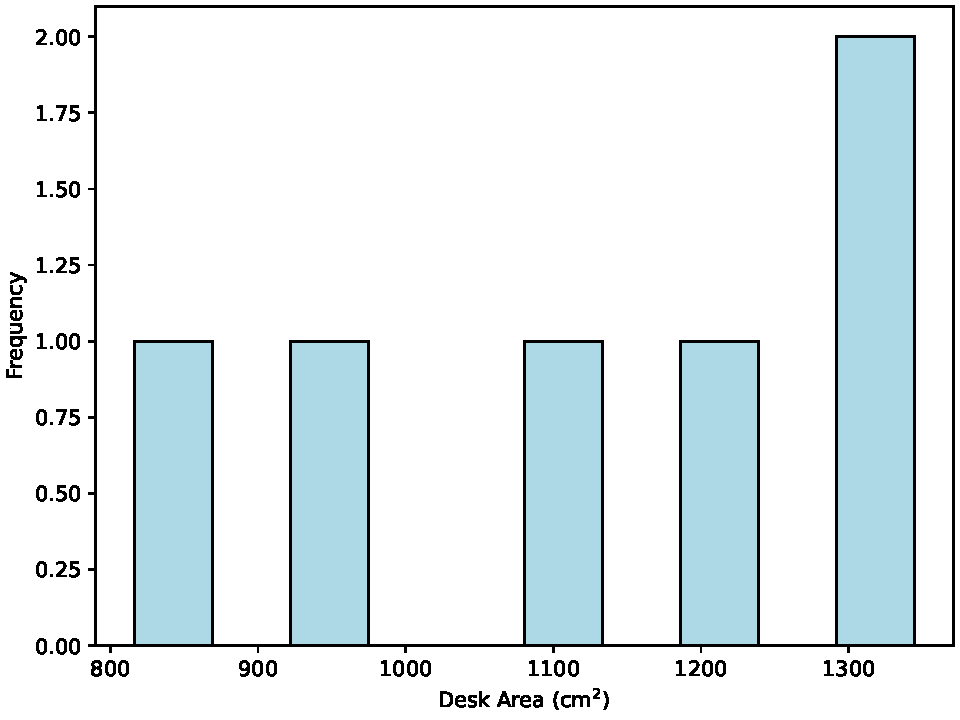
\includegraphics[width=\linewidth]{vis/hist.pdf}
\end{figure}

\pagebreak
\onecolumn

\subsection{Reproduced Figures from \cite{mohamed} \cite{Ansari}}

\begin{figure}[H]
    \centering
    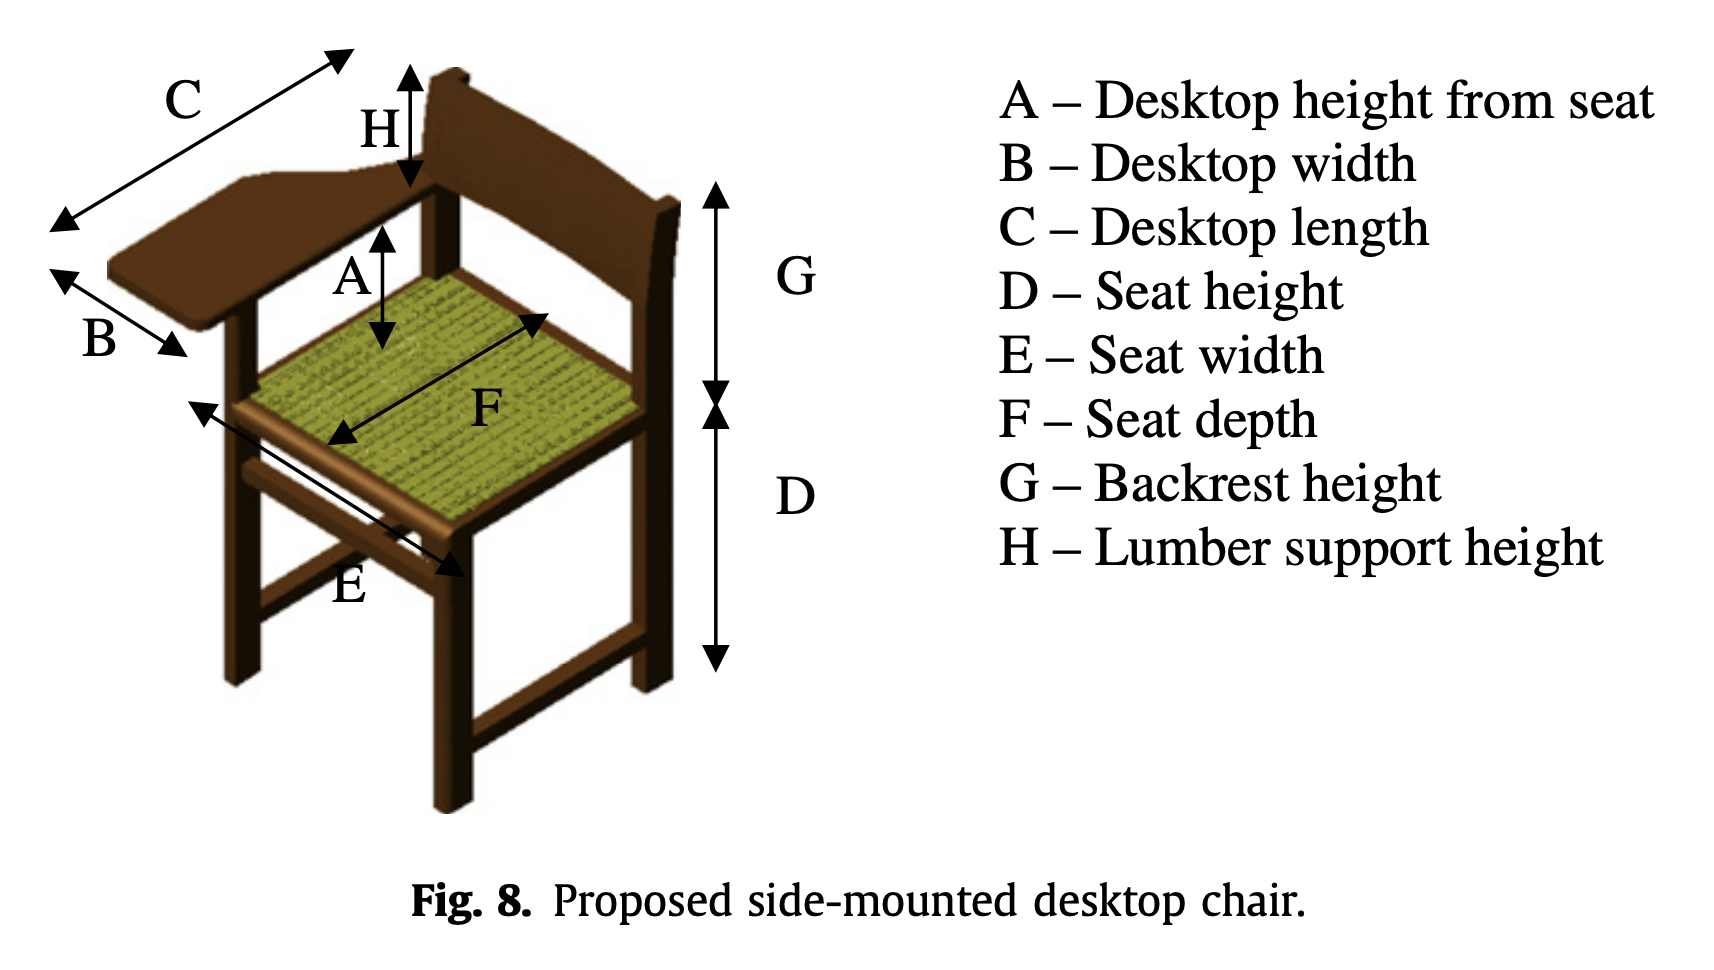
\includegraphics[width=0.6\linewidth]{vis/mohamed_chair.png}
\end{figure}

this ``figure 8'' is reproduced without permission from \cite{mohamed}. this is a representative 3d visualization of their optimal chair.

\begin{figure}[H]
    \centering
    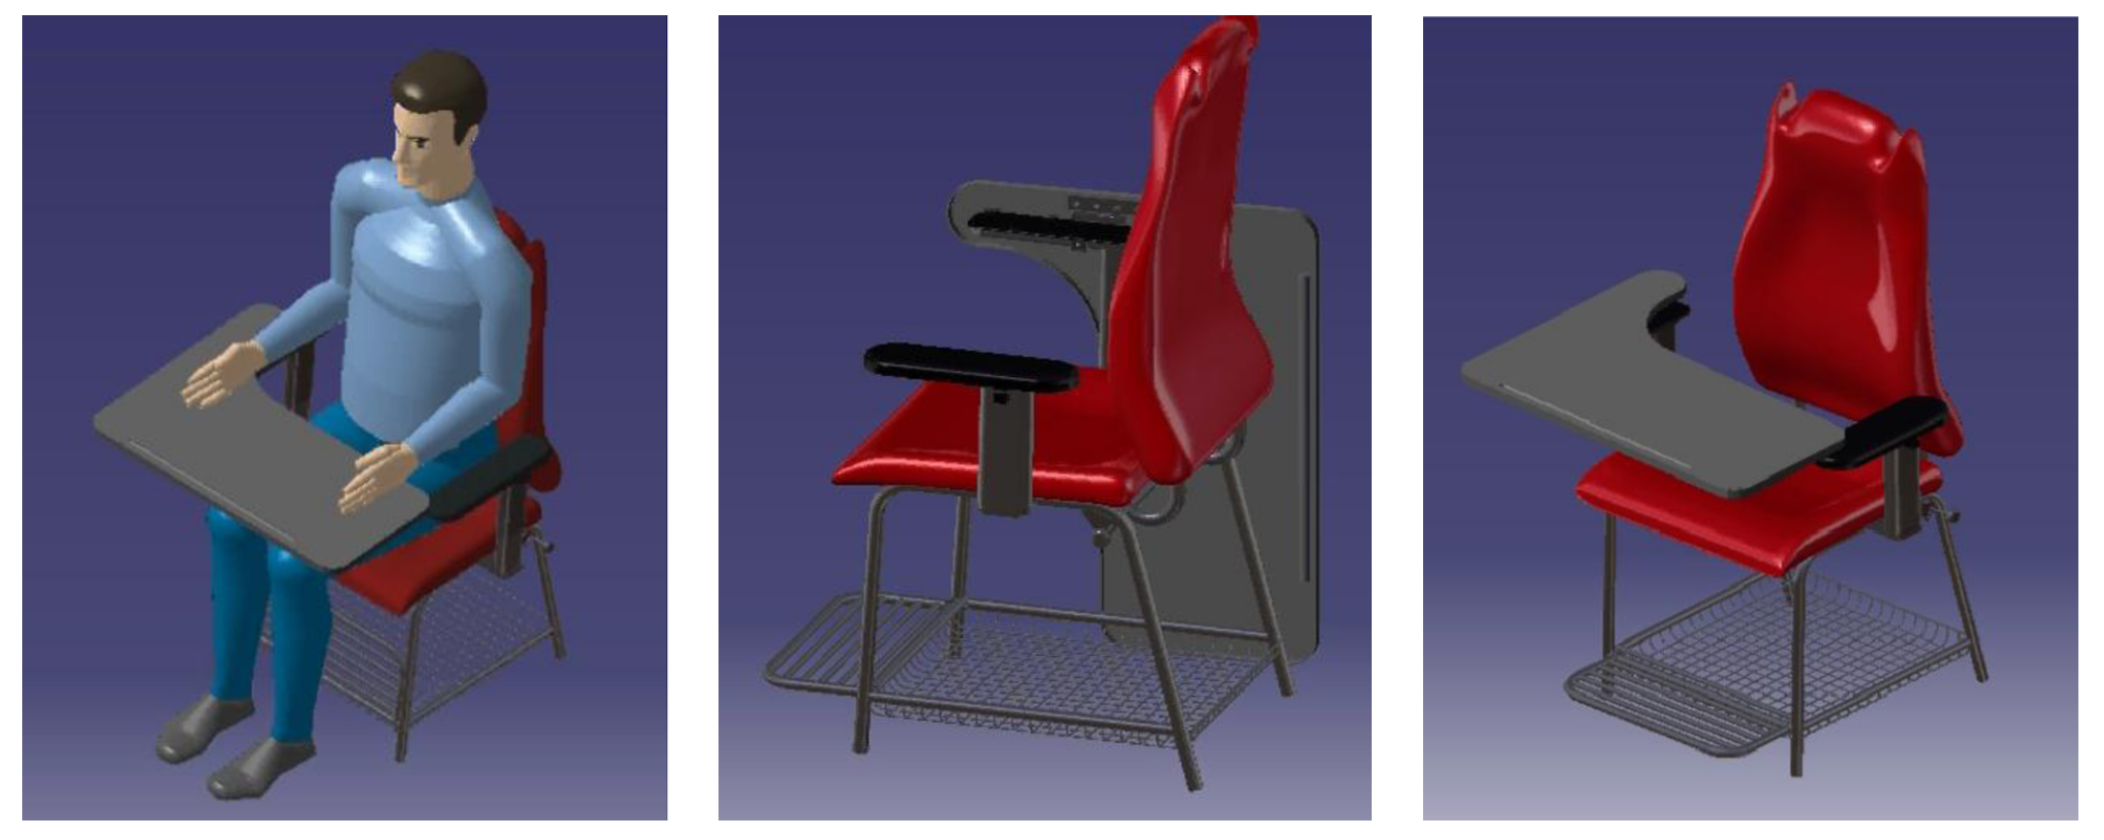
\includegraphics[width=0.6\linewidth]{vis/other_chair.png}
\end{figure}

this chair design is reproduced without permission from \cite{Ansari}. suprise suprise this is also a representitive 3d visualization of their optimal chair. but from 3 angles. 

\subsection{literally just all of our data}
see the next page for our data. it was originally collected in inches but was converted it into centimeters to make the comparison with literature a little easier for those who have trouble multiplying numbers by 2.54.


% sath group says unrotate

\clearpage
\onecolumn
\begin{tabular}{lrrrr}
    \toprule
    room & width (in) & length (in) & height from floor (in) & chair height (in) \\
    \midrule
    recitation hall 101 & 18.500000 & 11.187500 & 27.750000 & 17.375000 \\
    Smith Hall 209 & 12.500000 & 11.500000 & 28.750000 & 17.000000 \\
    Purnell Hall 115 & 10.125000 & 12.500000 & 23.500000 & 16.000000 \\
    Purnell Hall 227 & 16.500000 & 11.500000 & 28.000000 & 17.000000 \\
    Ewing Hall 204 & 18.125000 & 11.500000 & 27.000000 & 17.250000 \\
    Gore Hall 308 & 14.750000 & 11.750000 & 29.500000 & 18.250000 \\
    Penny 209 & 26.750000 & 23.500000 & 28.750000 & 17.750000 \\
    ISE 110 & 22.000000 & 12.250000 & 28.250000 & 18.000000 \\
    Pearson 114 & 21.500000 & 13.000000 & 29.000000 & 19.500000 \\
    Pearson 218 & 22.000000 & 12.250000 & 28.250000 & 18.000000 \\
    Colburn 366 & 10.130000 & 12.500000 & 27.000000 & 17.750000 \\
    Colburn 102 & 29.750000 & 17.500000 & 28.750000 & 17.750000 \\
    Colburn 109 & 14.630000 & 13.750000 & 27.750000 & 16.750000 \\
    Robinson 206 & 29.500000 & 19.750000 & 28.000000 & 16.250000 \\
    Robinson 203 & 34.500000 & 20.000000 & 30.000000 & 17.750000 \\
    Robinson 202 & 30.000000 & 24.000000 & 29.000000 & 17.750000 \\
    Memorial 37 & 16.750000 & 11.000000 & 28.000000 & 17.750000 \\
    Memorial 48 & 36.000000 & 36.000000 & 28.750000 & 16.750000 \\
    Memorial 28 & 9.600000 & 9.600000 & 28.500000 & 18.250000 \\
    Memorial 107 & 36.000000 & 21.000000 & 28.500000 & 18.250000 \\
    Memorial 110 & 28.000000 & 30.000000 & 28.750000 & 17.750000 \\
    Memorial 109 & 16.000000 & 26.000000 & 28.750000 & 18.250000 \\
    Memorial 127 & 28.250000 & 18.750000 & 31.500000 & 21.250000 \\
    Brown Lab 101 & 10.000000 & 11.500000 & 23.000000 & 16.250000 \\
    Brown Lab 116 & 13.000000 & 20.500000 & 29.000000 & 17.750000 \\
    Brown Lab 206 & 16.000000 & 26.000000 & 28.250000 & 17.750000 \\
    Brown Lab 220 & 29.750000 & 29.500000 & 28.750000 & 17.750000 \\
    Brown Lab 207 & 18.250000 & 11.625000 & 27.000000 & 18.500000 \\
    Gore Hall 102 & 18.250000 & 11.750000 & 28.250000 & 17.500000 \\
    Gore Hall 116 & 25.000000 & 22.000000 & 29.250000 & 19.500000 \\
    Gore Hall 218 & 22.000000 & 12.250000 & 28.250000 & 18.000000 \\
    Gore Hall 208 & 16.250000 & 11.250000 & 28.500000 & 16.250000 \\
    Gore Hall 304 & 14.750000 & 12.000000 & 29.750000 & 18.000000 \\
    Gore Hall 316 & 36.000000 & 36.000000 & 28.750000 & 16.750000 \\
    Sharp 100 & 14.500000 & 13.500000 & 28.500000 & 17.750000 \\
    Sharp 130 & 10.000000 & 11.500000 & 23.000000 & 16.250000 \\
    Wolf 100 & 10.000000 & 11.500000 & 23.000000 & 16.250000 \\
    Smith Hall 209 & 12.500000 & 11.500000 & 28.750000 & 17.000000 \\
    Smith Hall 120 & 10.000000 & 11.500000 & 23.000000 & 16.250000 \\
    Kirkbride 100 & 10.000000 & 11.500000 & 23.000000 & 16.250000 \\
    Ewing Hall 204 & 18.500000 & 11.500000 & 27.750000 & 17.250000 \\
    Purnell Hall 115 & 10.000000 & 11.500000 & 23.000000 & 16.250000 \\
    Purnell Hall 116 & 30.000000 & 24.000000 & 28.500000 & 17.250000 \\
    Purnell Hall 228 & 16.500000 & 11.500000 & 28.000000 & 17.000000 \\
    Purnell Hall 234 & 16.000000 & 26.000000 & 28.750000 & 18.250000 \\
    Purnell Hall 331 & 21.500000 & 13.000000 & 28.250000 & 18.500000 \\
    Alison 325 & 15.000000 & 13.750000 & 28.500000 & 17.250000 \\
    willard 208 & 19.410000 & 19.410000 & 29.125000 & 18.125000 \\
    willard 217 & 18.920000 & 18.920000 & 30.125000 & 18.625000 \\
    willard 218 & 18.920000 & 18.920000 & 30.125000 & 18.625000 \\
    willard 323 & 19.410000 & 19.410000 & 29.125000 & 18.125000 \\
    willard 319 & 19.410000 & 19.410000 & 29.125000 & 18.125000 \\
    \bottomrule
\end{tabular}    
\twocolumn
\clearpage



\end{document}
